%\documentclass[iop]{emulateapj}
\documentclass[aps, pre, onecolumn, nofootinbib, notitlepage, groupedaddress, amsfonts, amssymb, amsmath, longbibliography]{revtex4-1}
\usepackage{tabularx}
\usepackage{graphicx}
\usepackage{hyperref}
\usepackage{xcolor}
\hypersetup{
    colorlinks,
    linkcolor={red!50!black},
    citecolor={blue!50!black},
    urlcolor={blue!80!black}
}
\usepackage{bm}
\usepackage{natbib}
\usepackage{longtable}
\LTcapwidth=0.87\textwidth

\newcommand{\Div}[1]{\ensuremath{\nabla\cdot\left( #1\right)}}
\newcommand{\DivU}{\ensuremath{\nabla\cdot\bm{u}}}
\newcommand{\angles}[1]{\ensuremath{\left\langle #1 \right\rangle}}
\newcommand{\KS}[1]{\ensuremath{\text{KS}(#1)}}
\newcommand{\KSstat}[1]{\ensuremath{\overline{\text{KS}(#1)}}}
\newcommand{\grad}{\ensuremath{\nabla}}
\newcommand{\RB}{Rayleigh-B\'{e}nard }
\newcommand{\stressT}{\ensuremath{\bm{\bar{\bar{\Pi}}}}}
\newcommand{\lilstressT}{\ensuremath{\bm{\bar{\bar{\sigma}}}}}
\newcommand{\nrho}{\ensuremath{n_{\rho}}}
\newcommand{\approptoinn}[2]{\mathrel{\vcenter{
	\offinterlineskip\halign{\hfil$##$\cr
	#1\propto\cr\noalign{\kern2pt}#1\sim\cr\noalign{\kern-2pt}}}}}

\newcommand{\appropto}{\mathpalette\approptoinn\relax}

\newcommand\mnras{{MNRAS}}%

\begin{document}
\author{Evan H. Anders}
\affiliation{Dept. Astrophysical \& Planetary Sciences, University of Colorado -- Boulder, Boulder, CO 80309, USA}
\affiliation{Laboratory for Atmospheric and Space Physics, Boulder, CO 80303, USA}
\author{Benjamin P. Brown}
\affiliation{Dept. Astrophysical \& Planetary Sciences, University of Colorado -- Boulder, Boulder, CO 80309, USA}
\affiliation{Laboratory for Atmospheric and Space Physics, Boulder, CO 80303, USA}
\author{Jeffrey S. Oishi}
\affiliation{Department of Physics and Astronomy, Bates College, Lewiston, ME 04240, USA}
\title{Accelerated evolution of convective simulations}

\begin{abstract}
High Rayleigh number, turbulent convection is a classic system with a large timescale
separation between flow speeds and equilibration time.
In this paper, we present a method of achieving Accelerated Evolution (AE) of convective simulations which
fast-forwards through the long thermal evolution of these systems, and we test the
validity of this method. The AE procedure involves measuring the dynamics of convection
early in a simulation and using its characteristics to adjust the mean thermodynamic
profile within the domain towards its evolved state. We study \RB convection as a test case for AE.  
Key evolved properties of AE solutions are measured to be within a few percent
of measurements of the same quantities in solutions which are reached through 
evolution over a full thermal timescale. We conclude with a brief discussion of useful extensions
of AE, such as to studies of stratified, compressible convection.
\end{abstract}
\maketitle

%%%%%%%%%%%%
%%%%%%%%%%%
% INTRO
%%%%%%%%%%%
%%%%%%%%%%%%

\section{Introduction}
\label{sec:intro}
Astrophysical convection occurs in the presence of disparate timescales which
make direct numerical simulations of realistic models of systems in nature infeasible.  
Stiffness in astrophysical systems can manifest in multiple ways, some of which can
be handled by clever choices of numerical algorithms, and some which cannot.
For example,
flows in the convection zones of stars like the Sun are characteristically low Mach number
(Ma) in the deep interior. Initial value problems solved using
explicit timestepping methods are bound by the Courant-Friedrich-Lewy
(CFL) timestep limit corresponding to the fastest motions (sound
waves), resulting in timesteps which are prohibitively
small for studies of the deep, low-Ma motions. These systems are numerically
stiff, and the difference between
the sound crossing time and the convective overturn time have made studies of low-Ma stellar
convection difficult. This stiffness can be avoided using approximations such as
the anelastic approximation, in which sound waves are explicitly filtered out,
have been used to study low-Ma flows \cite{brown&all2010, featherstone&hindman2016}.
Recently, advanced numerical techniques which use fully implicit 
\cite{viallet&all2011, viallet&all2013, viallet&all2016} or mixed
implicit-explicit \cite{lecoanet&all2014, anders&brown2017, bordwell&all2018} 
timestepping mechanisms have made it feasible to study
convection in the fully compressible equations at low Mach numbers, 
and careful studies of deep convection which
would have been impossible a decade ago are now widely accessible.

Unfortunately, convective systems are stiff in more than one timescale and
generally evolve over the course of thermal
timescales, which are often much larger than all relevant
dynamical timescales. Transport by convection is a highly nonlinear process,
and this makes addressing the stiffness much more challenging; even fully
implicit  methods remain bound by the nonlinear flow timescales
\cite{viallet&all2011, viallet&all2013, viallet&all2016}. 
Resolving dynamics in atmospheres which are sufficiently
thermally relaxed remains a challenging problem.
Solar convection is a prime example of this phenomenon, as
dynamical timescales in the solar convective zone are relatively short 
(convection overturns every $\sim 5$ minutes at the solar surface)
compared to the Sun's Kelvin-Helmholtz timescale of
$3 \cdot 10^7$ years \cite{stix2003}.  
In such a system, it is impossible to resolve the convective dynamics while also
meaningfully evolving the thermal structure of the system using
traditional timestepping techniques alone.
As modern simulations aim to model natural convection
by in the high-Rayleigh-number (Ra) regime,
the thermal diffusion timescale becomes intractably large
compared to dynamical timescales \cite{anders&brown2017}, 
\begin{equation}
\frac{t_{\kappa}}{t_{\text{ff}}} = (\text{Ra Pr})^{1/2},
\end{equation}
where the thermal timescale is $t_{\kappa} = L_z^2 / \kappa$,
$L_z$ is the depth of the convective domain, $\kappa$ is
the thermal diffusivity, and
the freefall timescale is defined in Section \ref{sec:experiment}.
Furthermore, as dynamical and thermal timescales separate, 
simulations become more turbulent. Capturing appropriately resolved
turbulent motions requires finer grid meshes and smaller timesteps.
Thus, the progression of simulations into the high-Ra
regime of natural convection is slowed by two simultaneous effects: timestepping
through a single convective overturn time becomes more computationally expensive
and the number of overturn times required for systems to reach thermal equilibration
grows.

The vast difference between convective and thermal timescales has long plagued
numericists studying convection, and an abundance of approaches has been employed to
study thermally converged solutions. One popular method for accelerating the convergence
of high-Ra solutions is by ``bootstrapping'' -- the process of using the flow
fields in a converged solution at low Ra as initial conditions for a simulation at high
Ra.  This method has been used with great success \cite{johnston&doering2009, verzicco&camussi1997},
but it is not without its faults.  Bootstrapped solutions are susceptible to hysteresis
effects, in which large-scale convective structures present in the
low Ra solution imprint onto the dynamics of the new, high Ra solution. 
Another commonly-used tactic in
moderate-Ra simulations is to use a simplified system model to construct initial
conditions, such as the solution of a linear eigenvalue solve \cite{hurlburt&all1984} 
or an axisymmetric solution for convection in a 3D cylinder \cite{verzicco&camussi1997}. 
In other systems, a set of initial conditions closer to the evolved state than a standard
conductive state can be analytically derived \cite{couston&all2017, brandenburg&all2005};
these experiments all have slowly-evolving stable regions, and so a combination of
intuition from low-Ra solutions and established convective theory inform an
initial state which is closer to the evolved state than the standard conductive,
hydrostatic state often used.

Despite the numerous methods that have been used,
the most straightforward way to achieve a thermally converged solution
is to evolve a convective simulation through a thermal timescale. Some modern
studies do just that \cite{featherstone&hindman2016}.
Such evolution is computationally 
\emph{expensive}, and state-of-the-art simulations at the highest values of Ra
can only reasonably be run
for hundreds of freefall timescales \cite{stevens&all2011}, much less the
thousands or millions freefall times required for thermal convergence.

In this work, we study a method of achieving accelerated evolution of
convective simulations. We couple measurements of the dynamics of unequilibrated
convective simulations with knowledge about energy balances in the desired solution
to self-consistently adjust the mean vertical thermodynamic profile towards its evolved state. 
While a technique of this kind has been used previously \cite{hurlburt&all1986}.
The details of implementation, the convergence properties, and whether or not the
accelerated evolution state corresponds to a standard evolution state are not documented.
In section \ref{sec:experiment}, we describe our convective simulations, our
numerical methods, and the procedure for achieving accelerated evolution. In
section \ref{sec:results}, we compare accelerated evolution solutions
to solutions obtained from standard evolution through a full thermal diffusion timescale. Finally,
in section \ref{sec:extensions}, we offer concluding remarks and
discuss extensions of the methods presented here.


%%%%%%%%%%%%
%%%%%%%%%%%
% EXPERIMENT
%%%%%%%%%%%
%%%%%%%%%%%%

\section{Experiment}
\label{sec:experiment}
In this work we study a simple form of thermal convection:
incompressible \RB convection under the Oberbeck-Boussinesq approximation,
such that the fluid
has a constant kinematic viscosity ($\nu$), thermal diffusivity ($\kappa$), and coefficient
of thermal expansion ($\alpha$). The density of the fluid is a constant, $\rho_0$,
except in the buoyancy term, where it is $\rho = \rho_0(1  - \alpha T_1)$.
The gravitational acceleration, $\bm{g} = - g\hat{z}$, is constant.
The equations of motion are \cite{spiegel&veronis1960}:
\begin{gather}
\DivU = 0, 
	\label{eqn:incompressible}
\\
\frac{\partial \bm{u}}{\partial t} + \bm{u}\cdot\grad\bm{u} =
-\frac{1}{\rho_0}\grad P - g( 1 - \alpha T_1)\hat{z} + \nu\grad^2\bm{u}, 
	\label{eqn:dim_bouss_momentum}
\\
\frac{\partial T_1}{\partial t} + \bm{u}\cdot\grad(T_0 + T_1) = \kappa\grad^2 T_1,
	\label{eqn:dim_bouss_energy}
\end{gather}
where $\bm{u} = u\bm{\hat{x}} + v\bm{\hat{y}} + w\bm{\hat{z}}$ is the velocity, 
$T = T_0(z) + T_1(x, y, z, t)$ are the initial and fluctuating components of temperature, 
and $P$ is the kinematic pressure.
We non-dimensionalize these equations such that
length is in units of the layer height ($L_z$),
temperature is in units of the initial temperature jump across the layer ($\Delta T_0 = L_z \grad T_0$), 
and velocity is in units of the freefall velocity ($v_{\text{ff}} = \sqrt{\alpha g L_z^2 \grad T_0}$).
By these choices, one time unit is a freefall time ($t_{\text{ff}} = L_z/v_{\text{ff}}$).
We introduce a reduced kinematic pressure,
$\varpi \equiv (P / \rho_0 + \phi + |\bm{u}|^2 / 2) / v_{\text{ff}}^2$, where the gravitational
potential, $\phi$, is defined such that $\bm{g} = -\grad \phi$. 
In non-dimensional form, and substituting 
$\bm{u}\cdot\grad\bm{u} = \grad(|\bm{u}|^2/2) - \bm{u}\times(\grad\times\bm{u})$
and $\grad^2\bm{u} = -\grad\times\grad\times\bm{u}$, Eqns. \ref{eqn:dim_bouss_momentum} \& \ref{eqn:dim_bouss_energy}
become
\begin{align}
\frac{\partial \bm{u}}{\partial t} + \grad \varpi - T_1\hat{z} + \mathcal{R}\grad\times\bm{\omega} &= \bm{u}\times\bm{\omega},
	\label{eqn:bouss_momentum}
\\
\frac{\partial T_1}{\partial t} - \mathcal{P}\grad^2 T_1 + w \frac{\partial T_0}{\partial z} &= - \bm{u}\cdot\grad T_1,
	\label{eqn:bouss_energy}
\end{align}
where $\bm{\omega} = \grad \times \bm{u}$ is the vorticity.
The dimensionless control parameters $\mathcal{R}$ and $\mathcal{P}$ 
are set by the Rayleigh (Ra) and Prandtl (Pr) numbers,
\begin{equation}
\mathcal{R} \equiv \sqrt{\frac{\text{Pr}}{\text{Ra}}}, \qquad \mathcal{P} \equiv \frac{1}{\sqrt{\text{Pr}\,\text{Ra}}}, \qquad
\text{Ra} = \frac{g \alpha L_z^4 \grad T_0}{\nu\kappa} = \frac{(L_z\,v_{\text{ff}})^2}{\nu\kappa}, \qquad \text{Pr} = \frac{\nu}{\kappa}.
\end{equation}
We hold Pr $= 1$ constant throughout this work, such that $\mathcal{P} = \mathcal{R}$.
$\mathcal{P}$ and $\mathcal{R}$ are related to the inverse Reynolds and Peclet numbers of the
evolved flows.

In Eqns.~(\ref{eqn:incompressible}), (\ref{eqn:bouss_momentum}), \& (\ref{eqn:bouss_energy}),
linear terms are grouped on the left-hand side of the equations, while nonlinear terms
are found on the right-hand side. We timestep linear terms implicitly, and nonlinear
terms explicitly.
We utilize the 
Dedalus\footnote{\url{http://dedalus-project.org/}} 
pseudospectral framework \cite{burns&all2016} to evolve  
Eqns.~(\ref{eqn:incompressible}), (\ref{eqn:bouss_momentum}), \& (\ref{eqn:bouss_energy}) 
forward in time
using an implicit-explicit (IMEX), third-order, four-stage 
Runge-Kutta timestepping scheme RK443 \cite{ascher&all1997}.  

Variables are time-evolved on a dealiased Chebyshev (vertical)
and Fourier (horizontal, periodic) domain in which the
physical grid dimensions are 3/2 the size of the coefficient grid.  
We study 2D and 3D convection in which the domain is a cartesian box, 
whose dimensionless vertical extent is $z \in [-1/2, 1/2]$, 
and which is horizontally periodic with an extent of $x, y \in [0, \Gamma]$,
where $\Gamma = 2$ is the aspect ratio, as has been previously studied
\cite{goluskin&all2014, johnston&doering2009}. 
In 2D simulations, we set $v = \partial_y = 0$.
We specify no-slip, impenetrable boundary conditions at both the top and
bottom boundary,
\begin{equation}
u = v = w = 0 \, \, \text{at}\,\,z = \pm 1/2,
\label{eqn:vel_bcs}
\end{equation}
and we use mixed thermal boundary conditions, such that
\begin{equation}
T_1 = 0 \,\,\text{at}\,\, z=+1/2, \qquad
\frac{\partial T_1}{\partial z} = 0\,\,\text{at}\,\,z=-1/2.
\label{eqn:temp_bcs}
\end{equation}
For this choice of boundary conditions, the critical value of Ra at which
the onset of convection occurs is Ra$_{\text{crit}} = 1295.78$ \cite{goluskin2016}, and the
supercriticality of a run is defined as $S \equiv \text{Ra}/\text{Ra}_{\text{crit}}$.
Studies of convection which aim to model
astrophysical systems such as stars often employ mixed thermal
boundary conditions, as we do here \cite{hurlburt&all1984, cattaneo&all1991, korre&all2017}.
Our choice of the thermal boundary conditions in Eqn.~(\ref{eqn:temp_bcs}) 
was motivated by the fact that accelerated evolution is simpler when both the
thermal profile and the flux through the domain are fixed at some point in the domain.

The initial temperature profile is linearly unstable,
$T_0(z) = -z$. On top of this profile, we fill $T_1$ with
random white noise whose magnitude is $10^{-6}\mathcal{P}$, and which is
vertically tapered so as to match the thermal boundary conditions.
This ensures that the initial perturbations are much smaller than the
evolved convective temperature perturbations, even at large Ra.
We filter this noise spectrum in coefficient space, 
such that only the lower 25\% of the coefficients
have power; this low-pass filter is used to avoid populating the
highest wavenumbers with noise in order to improve the stability of our
spectral timestepping methods.


%%%%%%%%%%%%
%%%%%%%%%%%
% AE METHOD
%%%%%%%%%%%
%%%%%%%%%%%%

\section{The method of Accelerated Evolution}
\label{sec:ae}
Here we describe a method of Accelerated Evolution (AE), which we use 
to rapidly evolve the thermodynamic state of convective simulations.  
We compare this AE method to Standard Evolution
(SE), in which we evolve the atmosphere from noise initial conditions
for one thermal diffusion time,
$t_\kappa = \mathcal{P}^{-1}$. Both AE and SE simulations begin with identical
initial conditions, as described in section \ref{sec:experiment}.
As Ra increases, and $\mathcal{P}$ decreases, SE solutions become intractable, 
while the timeframe of convergence for an AE solution remains nearly constant
in simulation freefall time units (see table \ref{table:run_parameters}).

We study in depth a 2D simulation at $S = 10^5$ to demonstrate the power of AE.
We compare kinetic energy (KE, black line) and mean temperature (blue line)
traces from a SE run in Fig.~\ref{fig:time_trace}a to an AE run
in Fig.~\ref{fig:time_trace}c.
In Fig.~\ref{fig:time_trace}a, the time evolution of the SE simulation is shown.
The KE grows exponentially from white noise during the
first $\sim 25$ $t_{\text{ff}}$. The solution then saturates and begins to slowly
equilibrate towards the proper isothermal profile in the interior of the domain.
This slow equilibration is evident in the behavior of the blue line, which measures
$\angles{T} - T_{\text{top}}$, where \angles{T} is the volume-average of $T$, and
$T_{\text{top}} = -0.5$ is the temperature at the upper boundary.
The mean atmospheric temperature and
kinetic energies are fully converged when $t = 4000$ $t_{\text{ff}}$ $= 0.35$ $t_{\kappa}$.
We show roughly the first thousand freefall time
units of evolution, as well as the evolved thermodynamic state reached after a full
thermal time of evolution.  In Fig.~\ref{fig:time_trace}c, similar traces are
shown for the corresponding AE solution
at the same parameters. The same linear growth phase occurs, but shortly after
the peak of convective transient we accelerate the convergence of the atmosphere
through the process which we describe below. We adjust the 1D vertical profile of
the atmosphere three times, as denoted by the three labeled
arrows in the graph numbered 1-3.  After the third profile adjustment, we find that
the atmosphere is nearly in its converged state and we begin to sample the evolved
convective dynamics.

The horizontally averaged profiles of the vertical conductive flux, 
F$_{\kappa} = \angles{-\kappa\grad(T_0 + T_1)}_{x,y}$, and the vertical convective enthalpy flux,
F$_{\text{E}} = \angles{w(T_0 + T_1)}_{x,y}$, are the basis of the AE method.
Here we use $\angles{}_{x,y}$ to represent a horizontal average. We measure
both of these fluxes early in a simulation, retrieving profiles such as
those shown in Fig.~\ref{fig:time_trace}b.
As the atmosphere evolves towards
the isothermal profile specified by the upper (cold) boundary condition, excess
temperature throughout the atmosphere must leave the domain. This excess thermal
energy leaves through the upper boundary, as seen in 
Fig.~\ref{fig:time_trace}b, where the amount of flux exiting at the top of the domain
is nearly 20 times larger the flux entering the bottom of the domain. Once the atmospheric
temperature profile reaches its evolved state, the flux entering the bottom boundary
is equal to the flux exiting through the upper boundary.  In general, this 
evolution is slow in SE (Fig.~\ref{fig:time_trace}a), but AE (Fig. \ref{fig:time_trace}c)
can take a system whose fluxes are in a strongly disequilibrium state (Fig.~\ref{fig:time_trace}b),
and quickly put them into a near-equilibrium state, as shown in Fig.~\ref{fig:time_trace}d. In
this final state both boundaries conduct the same amount of flux.
The converged state achieved through AE is at most 5\% different from the SE solution, 
as shown in Fig.~\ref{fig:time_trace}e. 
This is a very small difference considering the short timescales on which convergence
is reached and the strongly disequilibrium state used to inform the AE process.

\begin{figure}[p!]
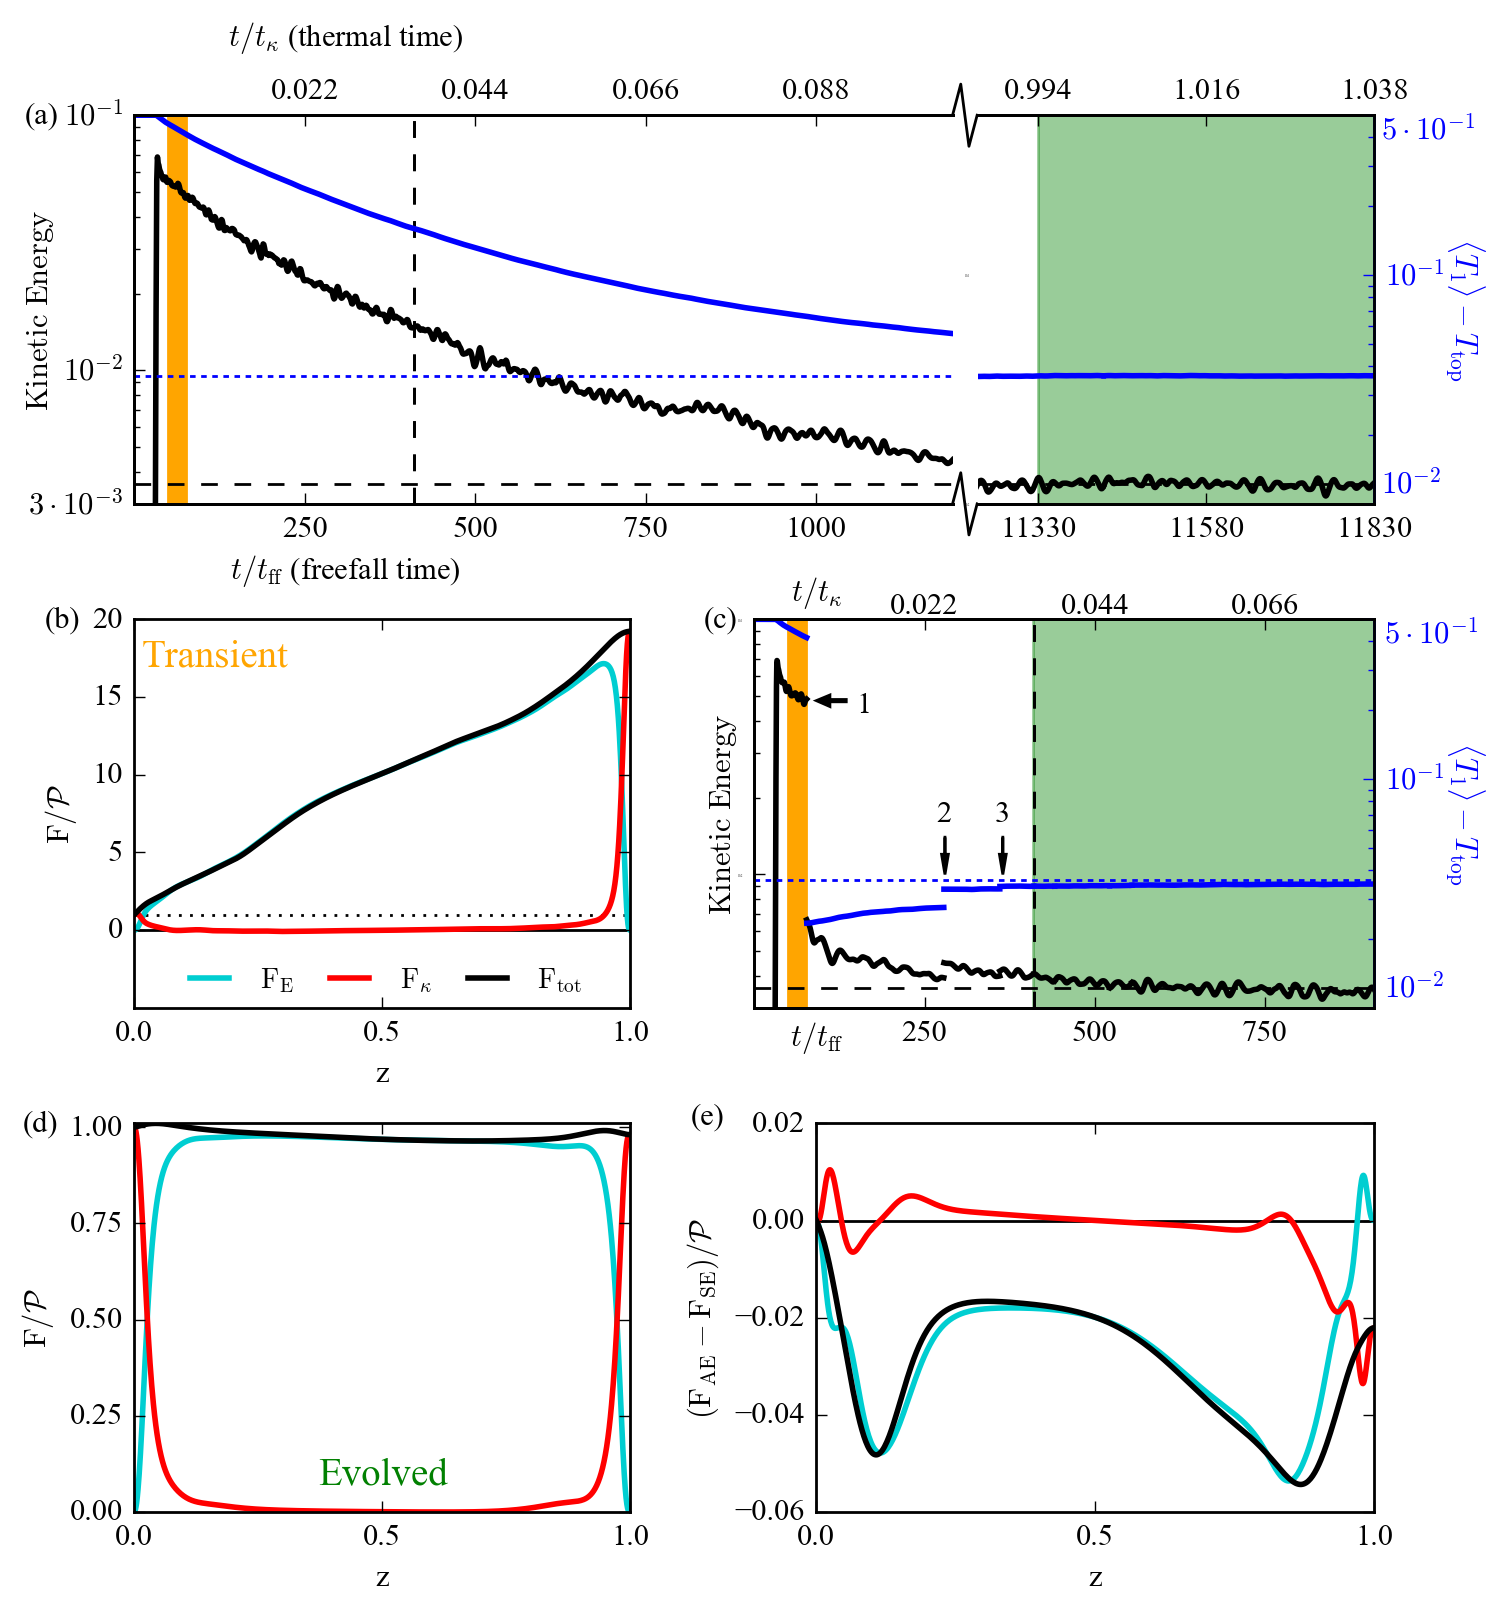
\includegraphics[width=\textwidth]{./figs/time_trace.png}
\caption{(a) Kinetic energy (black) and mean temperature (blue)  vs. time are shown
for a SE run at $S = 10^5$. The mean evolved values of kinetic energy and mean temperature,
averaged over the time shaded in green,
are denoted by the horizontal dashed lines. (b) The time- and horizontally-averaged
flux profiles are shown for the times highlighted in orange.
(c) The same quantities as in (a) are shown, but for AE at the same parameters.
The axes are scaled identically in (a) and (c), and the AE method is used three times, marked by
the numbered arrows in (c). The fluxes averaged over the green shaded region of (c)
are shown in (d). The difference between
the fluxes in the AE and SE solutions is shown in (e). \label{fig:time_trace} }
\end{figure}

In order to adjust the temperature profle to achieve AE, we calculate the total flux,
F$_{\text{tot}} =$ F$_{\text{E}}$ + F$_{\kappa}$, and then derive the profiles
\begin{equation}
f_{\text{E}}(z) = \frac{\text{F}_{\text{E}}}{\text{F}_{\text{tot}}},\qquad
f_{\kappa}(z) = \frac{\text{F}_{\kappa}}{\text{F}_{\text{tot}}},
\label{eqn:bvp_ratios}
\end{equation}
which have the systematic asymmetries (Fig.~\ref{fig:time_trace}b) removed. These profiles describe which
parts of the atmosphere depend on convection to carry flux (where $f_{\text{E}}(z) = 1$
and $f_{\kappa}(z) = 0$).
We presume that the early convection occupies roughly the same volume as the evolved
convection, and thus that the extent of the early thermal boundary layers 
(where $f_{\kappa}(z) = 1$ and $f_{\text{E}}(z) = 0$) 
will not change significantly over the course of the atmosphere's evolution.
Under this assumption, in order to reach the converged state, 
the flux through the atmosphere must be decreased by some amount,
\begin{equation}
\xi(z) \equiv \frac{\text{F}_{\text{B}}}{\text{F}_{\text{tot}}},
\label{eqn:xi}
\end{equation}
where $\text{F}_{\text{B}} = \mathcal{P}$ is the amount of flux that enters the
bottom of the atmosphere.

In a time-stationary state, the horizontal- and time-average of
Eqns.~(\ref{eqn:bouss_momentum}) and (\ref{eqn:bouss_energy}), neglecting terms which
vanish due to symmetry, are
\begin{gather}
\frac{\partial}{\partial z}\angles{\varpi}_{x,y} - \angles{T_1}_{x,y}\hat{z} = \angles{\bm{u}\times\bm{\omega}}_{x,y, \text{ ev}},
	\label{eqn:bouss_BVP_momentum}
\\
\frac{\partial}{\partial z}\text{F}_{\text{E, ev}} - \mathcal{P}\frac{\partial^2}{\partial z^2} \angles{T_1}_{x,y} = 0.
	\label{eqn:bouss_BVP_energy}
\end{gather}
Here, we construct $\angles{\bm{u}\times\bm{\omega}}_{x, y,\text{ ev}} =
\xi(z) \angles{\bm{u}\times\bm{\omega}}_{x, y}$ and $\text{F}_{\text{E, ev}} = \xi(z) \text{F}_{\text{E}}$
from our unevolved state, and solve for $\angles{\varpi}_{x,y}$ and $\angles{T_1}_{x,y}$.
Convective flows
are perturbations around a thermal profile defined by these equations in the proper evolved, 
statistically stationary state. Furthermore, under the specification of
F$_{\text{conv, ev}}$ and $\angles{\bm{u}\times\bm{\omega}}_{x,y\text{, ev}}$,
\emph{the mean thermodynamic structure of the system is fully specified}.

Thus, the AE method is simple: we pause a convective simulation and
construct $\xi(z)$ from measured flux profiles in the convective domain.
We solve a 1D boundary value problem consisting of
Eqns.~(\ref{eqn:bouss_BVP_momentum}) \& (\ref{eqn:bouss_BVP_energy})
to obtain the proper evolved thermodynamic profile, and proper conductive flux.
To obtain the proper convective enthalpy flux, we multiply both the velocity field,
$\bm{u}$, and the temperature perturbations around the mean profile, $T - \angles{T}_{x,y}$,
by $\sqrt{\xi}$, thus diminishing the magnitude of these perturbations appropriately.
After adjusing the fields of a simulation in this manner, we continue timestepping forward.
For specifics on the precise implementation of the AE method, we refer
the reader to appendix \ref{appendix:recipe}.


%%%%%%%%%%%%
%%%%%%%%%%%
% RESULTS
%%%%%%%%%%%
%%%%%%%%%%%%
\section{Results}
\label{sec:results}
We study evolved standard evolution (SE) solutions whose supercriticalities ($S$) are 
$S \in (1, 10^5]$ in 2D and $S \in (1, 10^4]$ in
3D. We compare their properties to
accelerated evolution (AE) runs at $S \in (1, 10^7]$ in 2D and
$S \in (1, 10^4]$ in 3D.
We refer the reader to appendix \ref{appendix:run_table} for a full list of
simulations.


The Nusselt number (Nu) quantifies the efficiency of convective heat transport
and is defined as
\begin{equation}
\text{Nu} = \frac{\angles{F_{\text{conv}} + F_{\text{cond}}}}{\angles{F_{\text{cond, ref}}}}
 = \frac{\angles{wT - \mathcal{P}\partial_z T}}{\angles{- \mathcal{P} \partial_z T}},
\end{equation}
where the volume average of a quantity, $\eta$, is shown as $\angles{\eta}$.
When $S < 10^{3+2/3}$ in 2D and for all runs in 3D, 
the evolved system is characterized by a time-stationary value of Nu, and is thus
in a state of constant convective heat transport.
At larger $S$ in 2D, the value of Nu varies significantly over time,
as shown by the time traces for $S = 10^5$ (top, left) and $S = 10^7$ (bottom, left) for two
AE runs in Fig.~\ref{fig:oscillating_plumes}. We find that these systems exhibit
large Nu during
states in which temperature fluctuations travel in their natural buoyant
direction (Fig.~\ref{fig:oscillating_plumes}, Ia \& IIa, where cold elements fall and hot elements rise).
However, when wrongly-signed temperature perturbations are entrained in an upflow or downflow
with oppositely signed fluid, Nu is suppressed (Fig.~\ref{fig:oscillating_plumes}, Ib and IIb, 
where warm fluid is pulled down by the downflow
lane, and cool fluid is drawn up by the upflow lane). The plumes in these
systems naturally oscillate over time, switching between transport being dominated
by a counterclockwise cell, as pictured in Fig.~\ref{fig:oscillating_plumes}, and
a counter-clockwise cell. Our choice of no-slip
boundary conditions prevents the fluid from entering a full domain shearing state 
\cite{goluskin&all2014}, and the
oscillatory nature of the plumes is stable.
The 2D SE simulations exhibit the same horizontally
oscillatory behavior as the AE solutions for the same initial conditions. 
This time-dependent behavior of Nu is not seen strongly in our 3D solutions,
however most 3D simulations we conducted were at low $S$ compared to the runs in
which this behavior was observed in 2D.

\begin{figure}[t!]
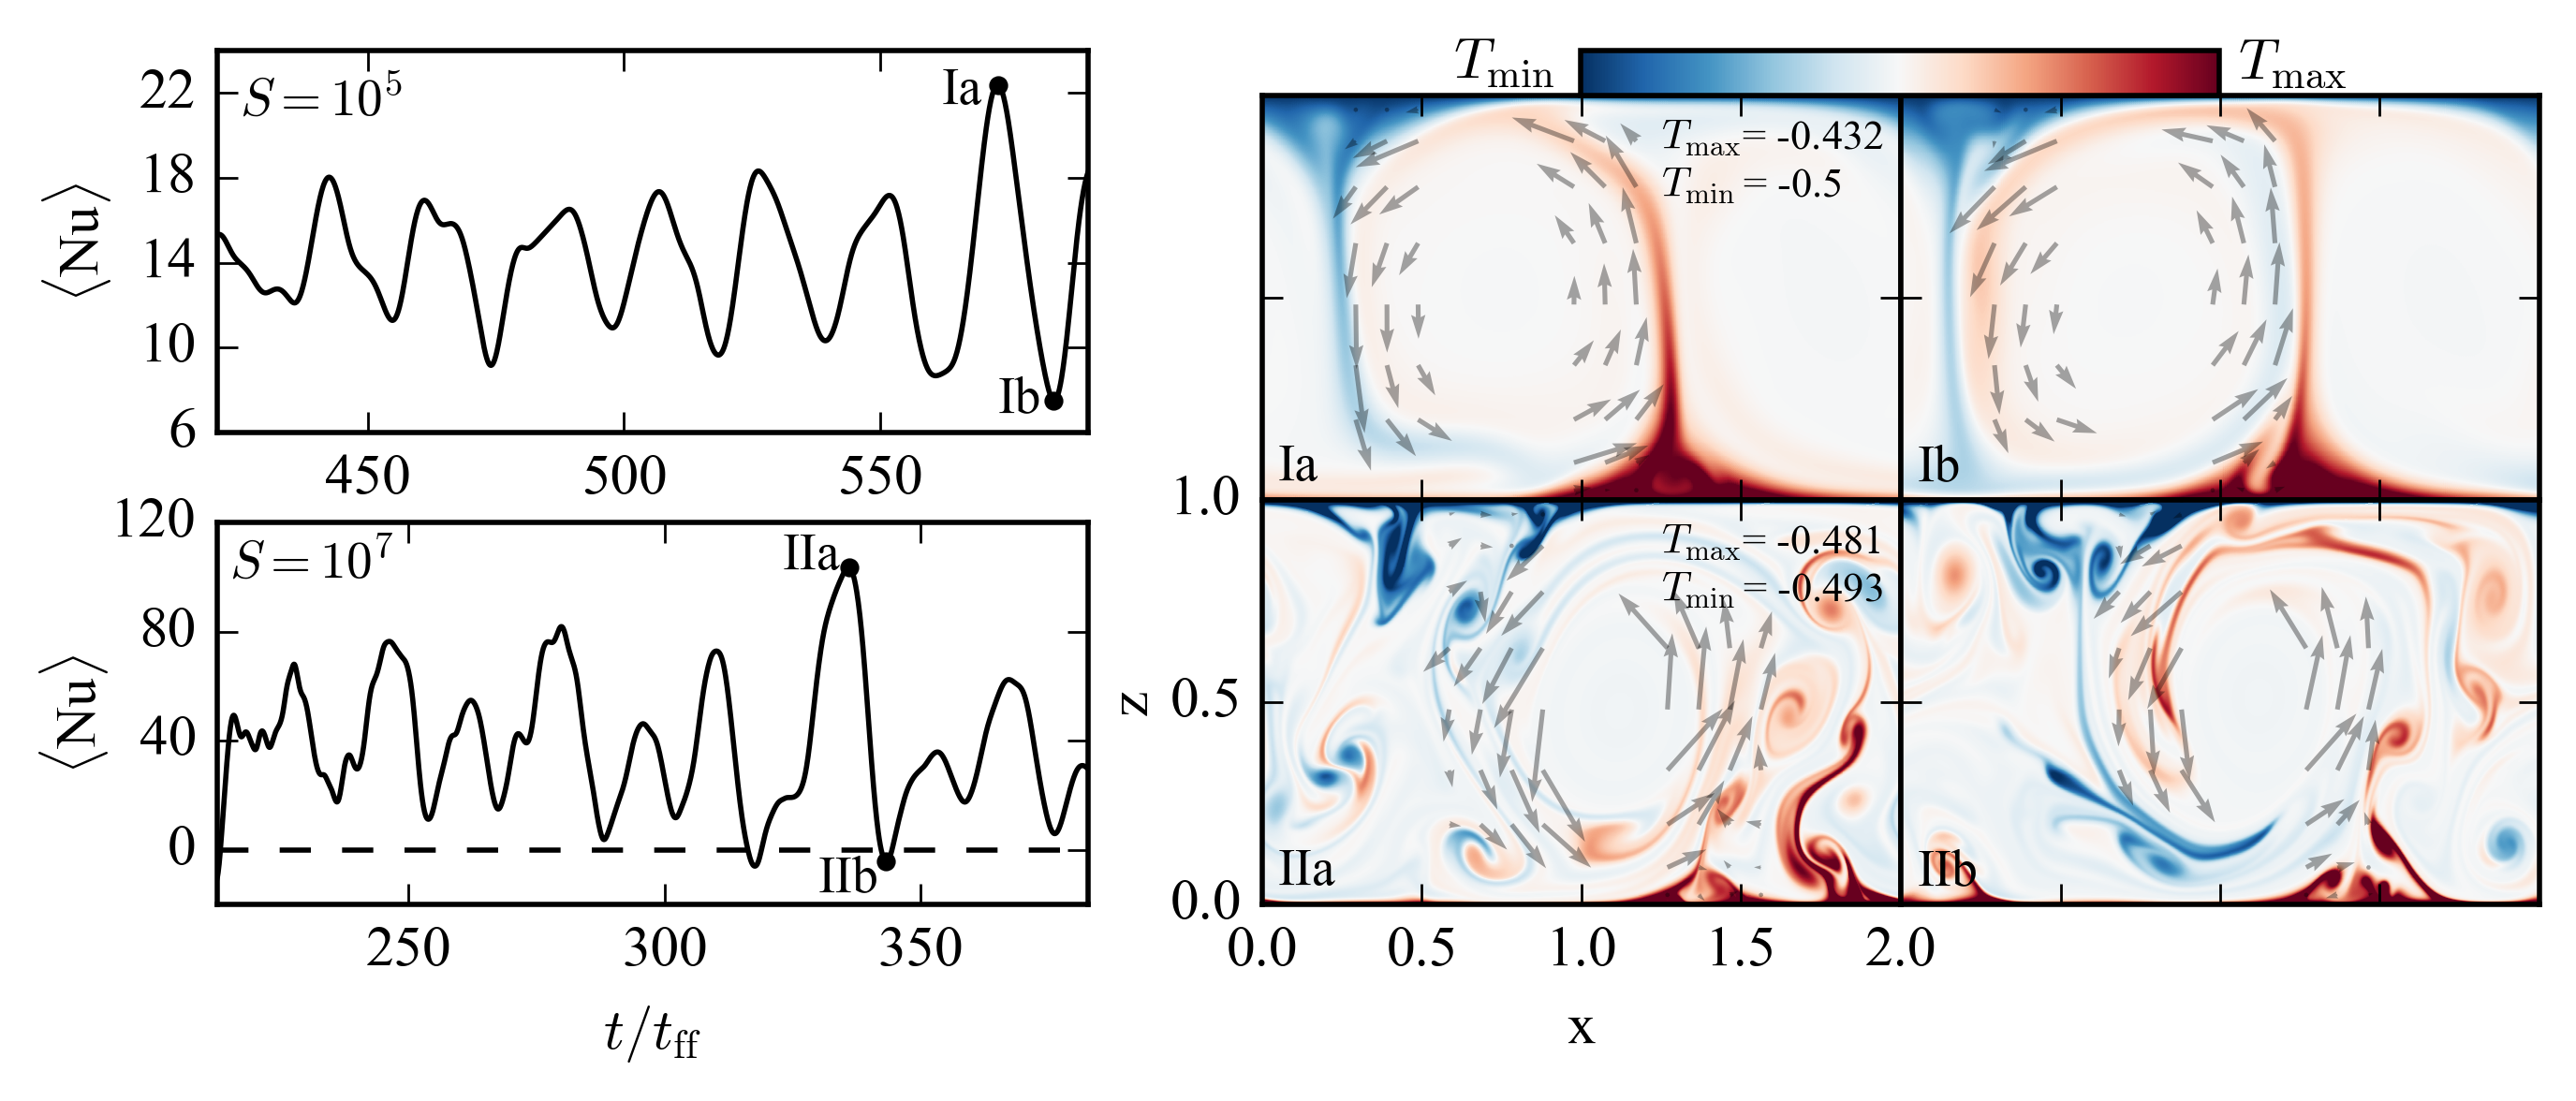
\includegraphics[width=\textwidth]{./figs/oscillating_plumes.png}
\caption{The time variation of the Nusselt number is shown for two AE cases at
$S = 10^5$ (top) and $S = 10^7$ (bottom). On the left, the instantaneous value of Nu
is shown as a function of time. On the right, temperature snapshots are shown for
Nu maxima (Ia \& IIa) and minima (Ib \& IIb). The suppressed value of Nu at the
minma arises from entrainment of fluid elements whose temperature perturbations
are wrongly signed (e.g., hot material going downwards and cold material going
upwards in Ib \& IIb). The colorbar scaling of panels Ia\&b are the same, as
are the scalings of panels IIa\&b. 
The minimum temperature is chosen by the fixed-temperature
boundary condition at the top, $T_{\text{top}} = -0.5$. The decreased range of
the colorbar scaling for
for IIa\&b was chosen to better display the convective dynamics.
\label{fig:oscillating_plumes} }
\end{figure}

\begin{figure}[b!]
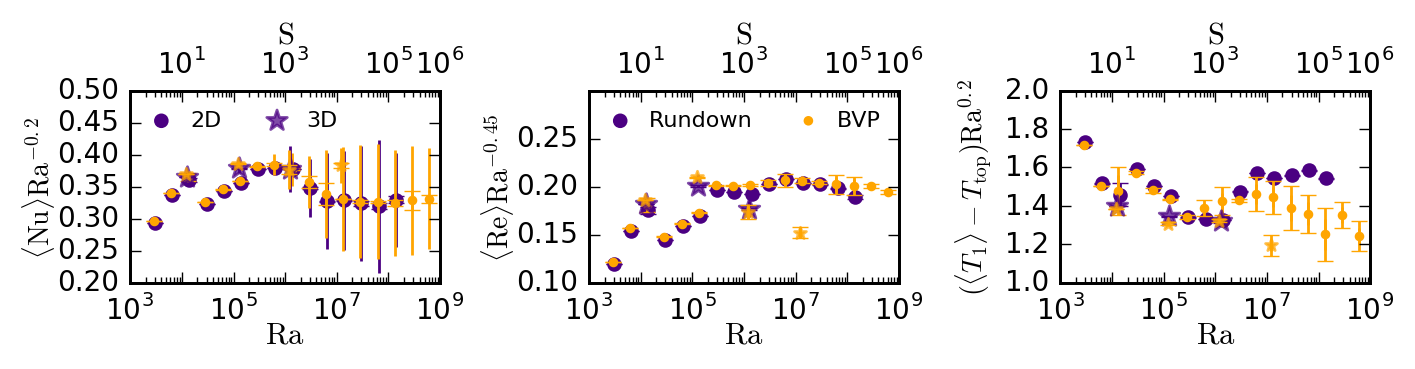
\includegraphics[width=\textwidth]{./figs/parameter_space_comparison.png}
\caption{Volume- and time-averaged measurements of the Nusselt number (Nu), the
RMS Reynolds number (Re), and the mean temperature ($\angles{T}$) for AE runs are shown in (a)-(c).
Symbols are located at the mean value of
each measurement and denote 2D (purple circles) and 3D (red stars). 
The run at $S = 10^5$ marked as a
black square is examined in more detail in Figs. \ref{fig:time_trace}, \ref{fig:oscillating_plumes},
\ref{fig:temp_comparison}, \& \ref{fig:pdf_comparison}.
Vertical lines represent the standard deviation of the measurement,
and quantify natural variation over the averaging window. 
(a) Nu scales as Ra$^{1/5}$; at high $S$ in 2D the value of Nu fluctuates over time
(see Fig.~\ref{fig:oscillating_plumes}).  
(b) Re, which measures turbulence in the solution, scales as
Ra$^{0.45}$. (c) The difference between $\angles{T}$ and the value of $T$ at the fixed-temperature
top boundary is shown; this quantity scales as Ra$^{-1/5}$, the inverse of Nu.
Relative error for measurements of (d) Nu, (e) Re, and (f) $\angles{T} - T_{\text{top}}$ between 
AE solutions and SE solutions are shown.
The greyed area of the plots indicates the region in which only AE runs were
carried out due to computational expense. \label{fig:parameter_space_comparison} }
\end{figure}




The time- and volume-averaged values of Nu, the RMS
Reynolds number (Re), and the mean temperature 
are shown for AE solutions in Fig.~\ref{fig:parameter_space_comparison}a-c.
Mean values are shown by the symbols (purple circles and red stars), and 
the vertical lines represent the standard deviation of the measurement over time.
Nu is shown as a function of Ra and $S$ in Fig.~\ref{fig:parameter_space_comparison}a.
The dynamic nature of the plume structures (e.g., Fig.~\ref{fig:oscillating_plumes})
diminishes the mean
scaling of the heat transport to $\text{Nu} \propto \text{Ra}^{1/5}$,
which is weaker than classic scaling laws \cite{johnston&doering2009, ahlers&all2009}.
Previous studies in 2D convection may have avoided these time-varying Nu states by using
bootstrapping techniques as initial conditions for high $S$ runs.
In Fig.~\ref{fig:parameter_space_comparison}b, we report 
$\text{Re} = \angles{|\bm{u}|} / \mathcal{R}$ as a function of Ra and $S$.  
Re measures the degree of
turbulence in the solution, and scales roughly as
$\text{Re} \propto \text{Ra}^{0.45}$. Each simulation shows little variance in
the value of Re over time.
Fig.~\ref{fig:parameter_space_comparison}c shows the scaling of $\angles{T} - T_{\text{top}}$,
the mean value of the temperature minus its value at the upper (fixed temperature) boundary.
The average temperature, $\angles{T}$, is dominated by its value in the isothermal interior,
so this measurements serves as a probe of the temperature jump across the boundary
layers. As a result, we expect this measure to
scale inversely with Nu in converged solutions
where fixed-flux boundary conditions are used \cite{otero&all2002}.  We find here
that $(\angles{T} - T_{\text{top}}) \propto \text{Ra}^{-1/5}$, precisely the inverse
scaling of Nu.



In Fig.~\ref{fig:parameter_space_comparison}d-f, we report the fractional difference
between measurements in the AE and SE solutions.
The mean values of Nu and $\angles{T} - T_{\text{top}}$ 
measured in AE are accurate to SE values to within $\sim 1$\%.
Re measurements show marginally greater error, with AE measurements being 
$\leq 2$\% different from SE measurements.

For the select 3D runs conducted in this study, the scaling of Nu, Re, and $\angles{T} - T_{\text{top}}$
reported in Fig.~\ref{fig:parameter_space_comparison}a-c is nearly identical to the
2D simulations. Errors between AE and SE solutions in 3D fall within the same range as
errors in 2D in Fig.~\ref{fig:parameter_space_comparison}d-f. AE is therefore
equally effective in both 2D and 3D, and we restrict much of our study to 2D here.

The measurements presented in Fig.~\ref{fig:parameter_space_comparison} demonstrate
that AE can be powerfully employed in parameter space studies in which
large numbers of simulations are compared in a volume-averaged sense.  We now turn
our examination to a more direct comparison of AE and SE for 2D convection at
$S = 10^5$, the time and flux evolution of which was shown in Fig.~\ref{fig:time_trace}.
All comparisons that follow for these two runs occur over the times shaded in
green in Fig.~\ref{fig:time_trace}a\&c. Measurements are sampled every
0.1 freefall time units for 500 total time units.

As AE is fundamentally a 1D adjustment to the thermodynamic structure of the
solution, we compare the horizontally- and time-averaged temperature profiles 
attained by AE and SE in Fig.~\ref{fig:temp_comparison}a.  
The boundary layer width and structure are  
nearly identical between the two solutions, but the
the mean temperature in the isothermal interior differs by roughly 0.5\%
(Fig.~\ref{fig:temp_comparison}c). 

\begin{figure}[t]
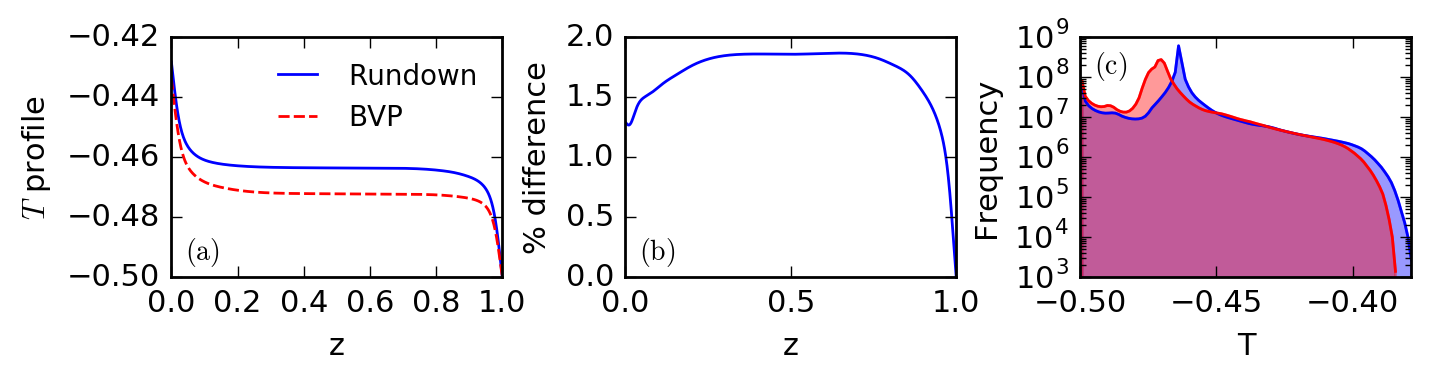
\includegraphics[width=\textwidth]{./figs/temp_comparison.png}
\caption{Comparisons of the evolved thermodynamic states of an AE and SE run
at $S = 10^{5}$ are shown.  (a) Evolved horizontally- and time-averaged 
temperature profiles, as a function of height.
(b) Probability Distribution Functions (PDFs) and their integrated
Cumulative Distribution Functions (CDFs)
of point-by-point measurements of the temperature field.
(c) The percentage difference between the mean temperature profiles as a function of height.
The difference between the mean profiles is very small, O(0.5\%).
(d) The value of the Kolmogorov-Smirnov (KS) statistic, or the difference between
the AE and SE CDFs, as a function of temperature.
The small
difference in the interior temperature 
results in a large difference between the two temperature CDFs near the values
of the temperature modes.  The spread of temperature around the modes, which includes the 
fluctuations that drive convection, are nearly identical between the two runs.
\label{fig:temp_comparison} }
\end{figure}

The probability distribution functions (PDFs)
of point-by-point temperature measurements are compared for the two runs
in Fig.~\ref{fig:temp_comparison}b. To construct these PDFs, 
we interpolate the full temperature field
at each measurement time onto an evenly spaced grid, determine the
frequency distribution of all $T$ values over the duration of the 500 $t_{\text{ff}}$
measurement window, and then normalize the
distribution such that its integral is unity.  The two PDFs have noticeably
different modes, as is expected from Fig.~\ref{fig:temp_comparison}a. 
Over long timescales, the 0.5\% difference between the two profiles would
disappear, as the AE solution evolves to be exactly the SE solution -- this
is evident in the asymmetry of the AE PDF near the mode
in Fig.~\ref{fig:temp_comparison}b and also
the trend of the mean temperature over time in Fig.~\ref{fig:time_trace}c.

One means of comparing two
PDFs to determine if they are drawn from the same underlying
sample distribution is through the use of a Kolmogorov-Smirnov (KS) test \cite{wall&jenkins2012}.
We calculate the KS statistic for a PDF of some value, $q$, as
\begin{equation}
\KS{q} = \text{CDF}_{\text{AE}}(q) - \text{CDF}_{\text{SE}}(q),
\label{eqn:ks_profile}
\end{equation}
where CDF stands for cumulative distribution function, the integral of the PDF.
A traditional Kolmogorov-Smirnov statistic is just a single value,
$\KSstat{q} = |\KS{q}|_\infty =
\text{max} |\KS{q}|$, and we use both the profile KS$(q)$ and
$\KSstat{q}$ to gain insight into the likeness of two PDFs. 
We show the $\KS{T}$ in Fig.~\ref{fig:temp_comparison}d, and the
CDFs used to construct it overlay the PDFs in Fig.~\ref{fig:temp_comparison}b.
Near the modes of the temperature PDFs, $\KSstat{T} = 0.495$, 
which is very large and implies that roughly half of all
measurements in the AE case are at a lower $T$ than those in the SE case.
While this difference is significant, it is also expected from Fig.~\ref{fig:temp_comparison}a.
Fortunately, $\KS{T}$ is very small away from the modes, 
indicating that the temperature fluctuations off of the modes, which are the primary
drivers of convective transport, are nearly identical.

In addition to comparing the thermodynamic state achieved by the SE and AE methods,
we examine the velocities and heat transport found in the evolved states.
Shown are the PDFs of 
vertical velocity ($w$, Fig.~\ref{fig:pdf_comparison}a), horizontal velocity ($u$, Fig. \ref{fig:pdf_comparison}b),
and the nonlinear vertical convective flux ($w(T - \angles{T}_{x,y})$, Fig.~\ref{fig:pdf_comparison}c). 
Each PDF here shows a strong peak near zero due to the no-slip, impenetrable
velocity boundary conditions (Eqn. (\ref{eqn:bcs})).
The CDFs of each profile are overplotted, and corresponding KS profiles are
shown in Fig.~\ref{fig:pdf_comparison}d-f.  We report
$\KSstat{w} = 0.00615$, $\KSstat{u} = 0.0349$,
and $\KSstat{w(T - \angles{T}_{x,y})} = 0.0263$.
The difference in vertical velocity
and heat transport between AE and SE is negligible, which is unsurprising in light of
the Nu measurements of Fig.~\ref{fig:parameter_space_comparison}a\&d.
this also confirms that the large $\KSstat{T}$ in Fig.~\ref{fig:temp_comparison}d is
not of concern, and that the AE run achieves the proper convective solution.
The horizontal velocity shows some small deviation between the two simulations, and this
likely relates to the precise configuration of the convective plumes (e.g., Fig.~\ref{fig:oscillating_plumes}).
We find that despite our no-slip boundary conditions, the full convective roll systems
migrate slowly to the left or the right over time, and the difference in $\KS{u}$
appears to be caused by a more prominent migration in the -x direction in the AE run
than in the SE run.


\begin{figure}[t]
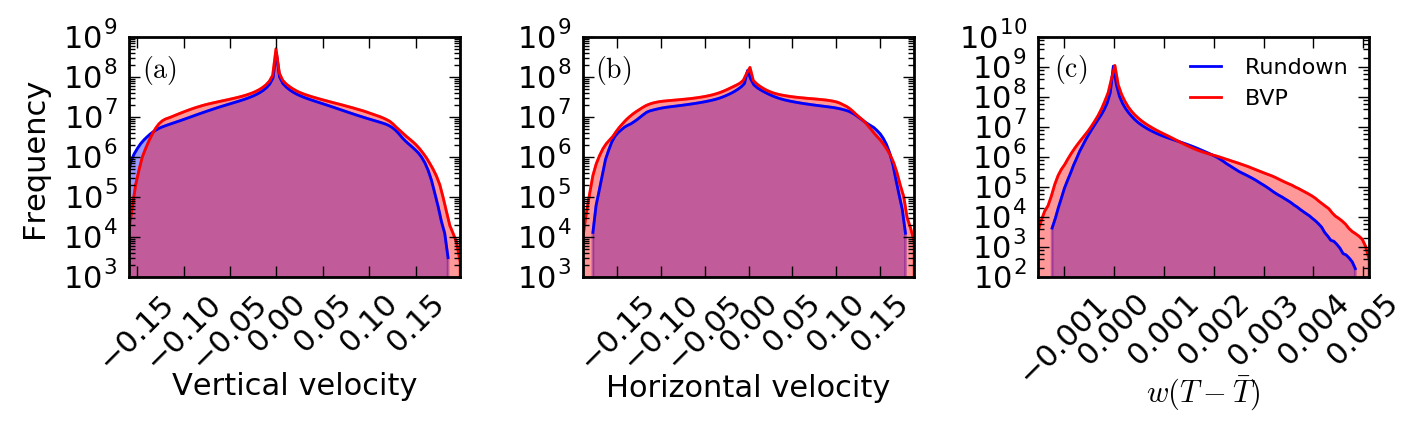
\includegraphics[width=\textwidth]{./figs/pdf_comparison.png}
\caption{Probability distribution functions (PDFs) of (a) the vertical velocity, (b) the horizontal velocity, and (c) nonlinear
convective transport are shown for 2D runs achieved through SE (blue) and AE (red)
at $S = 10^{5}$.  The cumulative distribution function (CDF) is overplotted for each PDF. 
(d-f) The KS profiles, as defined in Eqn. (\ref{eqn:ks_profile}),
are shown for the related distributions; solid lines indicate positive values
while dashed lines are negative values. Unlike the temperature distributions in
Fig.~\ref{fig:temp_comparison}, these distributions
show very good agreement and small values of the KS statistic.
\label{fig:pdf_comparison} }
\end{figure}


The small differences between the SE and AE solutions for the case studied in 
Figs. \ref{fig:time_trace}, \ref{fig:temp_comparison}, \& \ref{fig:pdf_comparison},
show the extreme power of AE.  In addition to the fact that AE runs require much
less total simulation time (see e.g., Fig.~\ref{fig:time_trace}a\&c and the time
values in the green highlighted regions), the first application of AE in a given
simulation (Fig.~\ref{fig:time_trace}c, at the arrow labeled ``1'') drastically
increases the average timestep by immediately progressing the simulation into
a more converged state. For the $S = 10^5$ case we examined in detail, the
average time step size grew by a factor of 2-3 due to the decreased convective
velocities from the transient state to the evolved state. 
At $S = 10^7$, the AE solve immediately improved the timestep size 
by nearly a factor of 4.
Thus, AE achieves converged solutions in few simulation time units,
while also taking less real world time per simulation time unit, when compared
to the slowly converging SE state at the same simulation time.


%%%%%%%%%%%%
%%%%%%%%%%%
% CONCLUSION
%%%%%%%%%%%
%%%%%%%%%%%%


\section{Extensions \& Conclusions}
\label{sec:extensions}
In this work we have studied a method of Accelerated Evolution (AE) which can
be employed to achieve rapid thermal convergence of convective simulations.  We compared
this technique to the Standard Evolution (SE) of convection through a full thermal diffusion timescale,
and we
showed that AE rapidly obtains solutions whose dynamics are statistically similar to SE solutions.
The AE method is valid at low values of $S$, where SE solutions
converge quickly due to the short thermal timescale, and AE remains applicable
at high values of $S$, where SE solutions are intractable.
As discussed, AE is equally applicable in 2D and 3D; here we have restricted most of our study to 2D
to extend our parameter space coverage.
At the largest values of $S$ in which AE and SE are compared in this work, we find
time savings of nearly an order of magnitude. 
For example, in 2D and at $S = 10^5$, the
AE run took 10.78 wall hours on 256 cores ($2.8\cdot 10^3$ cpu-hours) while the 
SE run took 94 wall hours ($2.4\cdot 10^4$ cpu-hours). In 3D and at $S = 10^4$,
the AE run took 2.81 wall hours on 8192 cores ($2.3 \cdot 10^4$ cpu-hours),
while the SE run took 37.9 wall hours, or ($3.1 \cdot 10^5$ cpu-hours). As $S$ increases,
and the thermal time, $t_{\kappa}$, simultaneously increases, we anticipate the 
computational and wall hour time
savings to further increase.  The increased computational expense of 3D runs compared
to 2D runs implies that 3D studies can greatly benefit from the proper implementation of AE.

Here we studied \RB convection as a test case for the AE method, but we argue that
the true power of this technique is in its extensions to more complicated studies.
To achieve AE in more complicated systems, one need only derive 
the steady-state, horizontally-averaged equations governing
the convective dynamics
(e.g., the analogs to Eqns.~(\ref{eqn:bouss_BVP_momentum}) \& (\ref{eqn:bouss_BVP_energy}))
and couple those equations with knowledge of the boundary conditions
and current dynamics as described in
section \ref{sec:ae} and appendix \ref{appendix:recipe}.
While in-depth studies of AE extensions are beyond the 
scope of this paper, we will briefly discuss
avenues in which the AE method should be explored and tested in order
to push these studies of different convective phenomena further into
the high-Ra regime.

Convection in natural systems is often driven by internal heating processes
rather than imposed, fixed boundary conditions. The AE procedure can be straightforwardly
applied to Boussinesq studies of internally heated convection \cite{goluskin2016},
where a constant source term in the energy equation causes 
the vertical flux through the system to increase with height.
In these systems, the thermal evolution is very slow compared to convective
dynamical timescales, just as it is in classic \RB convection.
These systems can be
studied using exactly the methods that we examined here, but 
multiplying the flux profiles derived
in Eqn. (\ref{eqn:bvp_ratios}) by the proper, height-dependent flux. Studies of
convection in natural system often employ height-dependent conductivities
\cite{brandenburg2016, kapyla&all2017}, leading
to natural flux divergences that act as internal heating terms.
The study
of AE in the context of simple internal heating simulations will be an important step
towards achieving AE in simulations with astrophysically realistic conductivities.
In these systems, the fluxes at the upper and lower boundaries are naturally different,
even in the evolved state. AE can rapidly adjust the thermal profile to carry the proper
amount of flux in and out of the domain, while achieving the proper interior isotherm.

A further area which could benefit from AE is overshooting convection, in which
studies examine adjacent stable and convecting regions
\cite{hurlburt&all1986, brandenburg&all2005, couston&all2017}.
When the interface between the stable region
and the convecting region is stiff,
convective motions cannot accelerate the restratification of the stable region.
In fully-convective domains, such as those studied in this work, the thermodynamics evolve
at a more rapid rate than the thermal diffusion time across the domain due to
convective mixing.  For example, in Fig.~\ref{fig:time_trace}a,
the SE solution is fully converged after $4\cdot 10^3$ frefall time units,
which is roughly 40\% of a thermal timescale. However, in 
studies where there is a stable region which is not mixed by convection, the experimentalist
must either wait through a thermal diffusion time for the region to restratify
or otherwise adjust the mean profile to study evolved atmospheres \cite{couston&all2017}.
In these systems, AE can instantaneously adjust the thermal profile in the
stable region from a far-disequilibrium state to the properly converged solution,
skipping the slow thermal evolution.

Studies of stratified, compressible convection have much to gain through
developing and employing AE.
In many studies of stratified convection, the thermal diffusivity
is a non-constant coefficient and varies
inversely proportional to the density \cite{anders&brown2017}. Thus, the
thermal timescale grows with depth in the atmosphere, and
the difficulty of achieving thermal convergence grows as simulators study more highly
stratified domains. For example, in a modestly stratified atmosphere which spans three
density scale heights, the density at the bottom, and thus the thermal timescale, is a
factor of 20 greater than at the top of the domain.
In order to extend AE into this regime, two additional pieces of information must be considered.
First, rather than constructing the profiles in Eqn. (\ref{eqn:bvp_ratios})
with the total flux through the domain, only the superadiabatic portion of
the flux should be considered \cite{anders&brown2017}.
Second, in addition to solving for
hydrostatic balance and thermal equilibrium, as in Eqns. (\ref{eqn:bouss_BVP_momentum})
\& (\ref{eqn:bouss_BVP_energy}), it is essential to simultaneously evolve the density
profile in a manner which conserves mass.  In a 1D boundary value problem, such as
is solved to achieve AE here, this implies the inclusion of an equation which tracks
the vertically integrated mass, and sets boundary conditions on that mass to ensure
that no mass enters or leaves the domain.

AE techniques can contribute to improving the description of convection
in stellar evolution codes. Current state of the art stellar structure
models are the solutions of 1D simulations which parameterize convection 
using Mixing Length Theory and its variants
\cite{paxton&all2011, paxton&all2013, paxton&all2015, paxton&all2018}. 
Recent studies \cite{viallet&all2011, viallet&all2013, viallet&all2016, arnett&all2015, cristini&all2016}
have tried
to understand how to simultaneously resolve convective motions and evolve
systems through many thermal timescales, as is required when determining the
interior structure of stars over their evolving lifetimes.
We now know that implicit timestepping methods
must resolve convective motions in order to timestep with stability
\cite{viallet&all2011, viallet&all2013, viallet&all2016}, and thus
cannot achieve fast, meaningful system evolution.
Other efforts have begun to project the results of 3D simulations into 1D
models to more properly parameterize convection for stellar evolution
\cite{arnett&all2015, cristini&all2016}, but the validity of these 321D techniques
has not been hitherto thoroughly tested. This is precisely the technology
employed in the tested AE method we present here. Through the careful expansion
of AE from \RB convection to fully stratified, compressible convection with realistic
opacities, it is possible that carefully evolved stellar structure models which
use statistics from resolved convective motions, rather than parameterized 1D models,
are well within reach of modern computing tools.

\begin{acknowledgments}
EHA acknowledges the support of the University of Colorado's George 
Ellery Hale Graduate Student Fellowship.
This work was additionally supported by  NASA LWS grant number NNX16AC92G.  
Computations were conducted 
with support by the NASA High End Computing (HEC) Program through the NASA 
Advanced Supercomputing (NAS) Division at Ames Research Center on Pleiades
with allocations GID s1647 and GID g26133.
\end{acknowledgments}


\appendix
\section{Accelerated Evolution Recipe}
\label{appendix:recipe}
In order to achieve Accelerated Evolution (AE), we pause the Direct Numerical Simulation (DNS)
which is evolving the dynamics of convection and solve a 1D Boundary Value Problem (BVP)
consisting of Eqns. (\ref{eqn:bouss_BVP_momentum}) \& (\ref{eqn:bouss_BVP_energy}).
After solving this BVP, we appropriately adjust the fields being evolved in the DNS
towards their evolved state, and then we continue running the now-evolved DNS.
The specific steps taken in completing the AE method are as follows:
\begin{enumerate}
\item Wait some time, $t_{\text{transient}}$, before beginning the AE process.
\item During the DNS, calculate time averages of the 1D vertical profiles of
F$_{\text{E}}$, F$_{\text{tot}}$, 
and $\angles{\bm{u} \times \bm{\omega}}_{x,y}$, updating them every timestep.  
To calculate these
averages, we use a trapezoidal-rule integration in time, and then divide by the
total time elapsed over which the average is taken. 
\item Pause the DNS once the averages are sufficiently converged. 
To ensure that an average is converged, at
least some time $t_{\text{min}}$ must have passed since the average was started to
ensure that the full range of convective dynamics are probed, and
the profiles must change by no more than $P$\% on a given timestep.
\item Construct $\xi$, F$_{\text{E, ev}}$, and $\angles{\bm{u} \times \bm{\omega}}_{x,y\text{, ev}}$,
as specified in section \ref{sec:ae}
from the averaged profiles.
\item Solve the BVP for $\angles{T_1}_{x,y}$ and $\angles{\varpi}_{x,y}$ of the
evolved state.  Set the horizontal average of the current DNS thermodynamic fields
equal to the results of the BVP.
\item Multiply the velocity field, $\bm{u} = u\hat{x} + v\hat{y} + w\hat{z}$,
and the temperature fluctuations, $T - \angles{T}_{x,y}$,
by $\sqrt{\xi}$ in the DNS to properly reduce the convective flux.
\item Continue running the DNS.
\end{enumerate}
We refer to this process as an ``AE BVP solve.''

While the use of a single AE BVP solve rapidly advances the convecting state to
one that is closer to the evolved state, we find that repeating this method 
multiple times is the best way to
ensure that the AE solution is truly converged. For all runs in 2D at $S < 10^5$, we
set $t_{\text{transient}} = 50$, completed an AE BVP solve
with $t_{\text{min}} = 30$ and $P = 0.1$, and then repeated the procedure.
For all 3D runs and 2D runs with $S \in [10^5, 10^6]$,
we did a first AE BVP solve with $t_{\text{transient}} = 20$,
$t_{\text{min}} = 20$, and $P = 1$ in order to quickly reach a near-
converged state and vastly increase our timestep size.  After this first solve, 
we completed two AE BVP solves, with $t_{\text{transient}} = 30$,
$t_{\text{min}} = 30$, 
and $P = 0.1$ to get very close to the solution (as in Fig.~\ref{fig:time_trace}c).
At very high $S = 10^7$, we ran two AE BVP solves with $t_{\text{min}} = 20$ and
$P = 1$. For the first solve, we set $t_{\text{transient}} = 20$, and for the
second we set $t_{\text{transient}} = 30$. We used fewer solves at this high
value of $S$ in part to reduce the computational expense of the run, and in
part because a third BVP generally did not greatly alter the solution
(as in Fig.~\ref{fig:time_trace}c, arrow 3). We wait 50 freefall times after
the final AE BVP solve of each run before beginning to take measurements.




\section{Table of Runs}
\label{appendix:run_table}
In Table \ref{table:run_parameters} we list key properties of all simulations
conducted in this work.  
\begin{table}
\caption{Simulation parameters. We report the supercriticality ($S$), Rayleigh number (Ra), 
and coefficient resolution (nz, nx, and ny are the number of coefficients in the
z, x, and y directions respectively).
Simulation run times required to reach convergence
are reported for the SE solutions ($t_{\text{therm}}$) and the AE solutions ($t_{\text{AE}}$).
The amount of time over which simulations measurements were taken in the evolved
state is listed ($t_{\text{avg}}$). All times are in freefall time units.  
The volume-averaged Nusselt number (Nu) of the
AE and SE solutions are shown.
In the upper part of the table, information pertaining to 2D runs is reported,
while information pertaining to 3D runs is in the lower part of the table.
}
\label{table:run_parameters}
\begin{center}
\begin{tabularx}{\textwidth}{ X X X X | X X X | X X }
\hline																	
$S$	&	Ra	&	nz	&	nx, ny	&	$t_{\text{therm}}$	&	$t_{\text{AE}}$	&	$t_{\text{avg}}$	&	Nu$_{\text{SE}}$	&	Nu$_{\text{AE}}$	\\
\hline \hline \multicolumn{9}{c}{\vspace{-0.2cm}}\\
\multicolumn{9}{c}{\vspace{0.1cm}2D Runs} \\
\hline
$10^{1/3}$	&	$2.79 \cdot 10^3$	&	32	&	64	&	$52.8$	&	$340$	&	100	&	1.46	&	1.46	\\
$10^{2/3}$	&	$6.01 \cdot 10^3$	&	32	&	64	&	$77.6$	&	$282$	&	100	&	1.95	&	1.95	\\
$10^1$	&	$1.30 \cdot 10^4$	&	32	&	64	&	$114$	&	$265$	&	100	&	2.43	&	2.42	\\
$10^{1 + 1/3}$	&	$2.79 \cdot 10^4$	&	32	&	64	&	$167$	&	$251$	&	100	&	2.54	&	2.54	\\
$10^{1 + 2/3}$	&	$6.01 \cdot 10^4$	&	32	&	64	&	$245$	&	$245$	&	100	&	3.14	&	3.14	\\
$10^2$	&	$1.30 \cdot 10^5$	&	64	&	128	&	$360$	&	$326$	&	100	&	3.8	&	3.8	\\
$10^{2 + 1/3}$	&	$2.79 \cdot 10^5$	&	64	&	128	&	$528$	&	$248$	&	100	&	4.71	&	4.71	\\
$10^{2 + 2/3}$	&	$6.01 \cdot 10^5$	&	64	&	128	&	$776$	&	$251$	&	100	&	5.5	&	5.5	\\
$10^3$	&	$1.30 \cdot 10^6$	&	128	&	256	&	$1.14 \cdot 10^3$	&	$268$	&	200	&	6.4	&	6.33	\\
$10^{3 + 1/3}$	&	$2.79 \cdot 10^6$	&	128	&	256	&	$1.67 \cdot 10^3$	&	$247$	&	500	&	6.87	&	6.95	\\
$10^{3 + 2/3}$	&	$6.01 \cdot 10^6$	&	256	&	512	&	$2.45 \cdot 10^3$	&	$275$	&	500	&	7.54	&	7.59	\\
$10^4$	&	$1.30 \cdot 10^7$	&	256	&	512	&	$3.60 \cdot 10^3$	&	$301$	&	500	&	8.83	&	8.83	\\
$10^{4 + 1/3}$	&	$2.79 \cdot 10^7$	&	256	&	512	&	$5.28 \cdot 10^3$	&	$317$	&	500	&	10.13	&	10.14	\\
$10^{4 + 2/3}$	&	$6.01 \cdot 10^7$	&	256	&	512	&	$7.76 \cdot 10^3$	&	$326$	&	500	&	11.65	&	11.69	\\
$10^5$	&	$1.30 \cdot 10^8$	&	512	&	1024	&	$1.14 \cdot 10^4$	&	$411$	&	500	&	14.02	&	14.18	\\
$10^{5 + 1/3}$	&	$2.79 \cdot 10^8$	&	512	&	1024	&	$1.67 \cdot 10^4$	&	$391$	&	500	&	---	&	16.21	\\
$10^{5 + 2/3}$	&	$6.01 \cdot 10^8$	&	512	&	1024	&	$2.45 \cdot 10^4$	&	$453$	&	500	&	---	&	18.58	\\
$10^6$	&	$1.30 \cdot 10^9$	&	1024	&	2048	&	$3.60 \cdot 10^4$	&	$436$	&	500	&	---	&	22.13	\\
$10^7$	&	$1.30 \cdot 10^{10}$	&	2048	&	4096	&	$1.14 \cdot 10^5$	&	$183$	&	170	&	---	&	38.29	\\
\\ \hline \hline \multicolumn{9}{c}{\vspace{-0.2cm}}\\
\multicolumn{9}{c}{\vspace{0.1cm}3D Runs} \\
\hline
$10^1$	&	$1.30 \cdot 10^4$	&	32	&	64$\times$64	&	$114$	&	$261$	&	100	&	2.42	&	2.42	\\
$10^2$	&	$1.30 \cdot 10^5$	&	64	&	128$\times$128	&	$360$	&	$249$	&	100	&	3.97	&	4	\\
$10^3$	&	$1.30 \cdot 10^6$	&	128	&	256$\times$256	&	$1.14 \cdot 10^3$	&	$243$	&	500	&	6.27	&	6.27	\\
$10^4$	&	$1.30 \cdot 10^7$	&	256	&	512$\times$512	&	$3.60 \cdot 10^3$	&	$244$	&	500	&	9.92	&	9.88	\\
\hline																	
\end{tabularx}
\end{center}
\end{table}





\bibliography{biblio.bib}
\end{document}
